% Source: tex/chapters/ch05/04_ソフトウェアテストの基礎.tex
\subsubsection{欠陥と障害}
欠陥は、望ましくない振る舞いの原因である。障害は、その原因が実行時に表に出て、利用者や外部システムから観測される現象である。欠陥があっても、該当する入力や状態に到達しなければ障害として現れないことがある。逆に、障害が観測されても、どの欠陥が原因かを一意に決められるとは限らない。

テストが直接明らかにするのは、多くの場合、障害である。テストに失敗した後は、デバッグや原因分析によって欠陥を見つけ、修正する必要がある。したがって、「テスト」と「デバッグ」は連続して使われることが多いが、同じ活動ではない。テストは失敗を検出する活動であり、デバッグは原因を突き止めて直す活動である。

\begin{pointbox}{重要}
テストは、欠陥の存在を示すことはできるが、欠陥が存在しないことを一般には証明できない。現実のソフトウェアでは、完全な網羅テストが不可能だからである。
\end{pointbox}

\begin{figure}[htbp]
\centering
\IfFileExists{assets/fig-ch05-03.png}{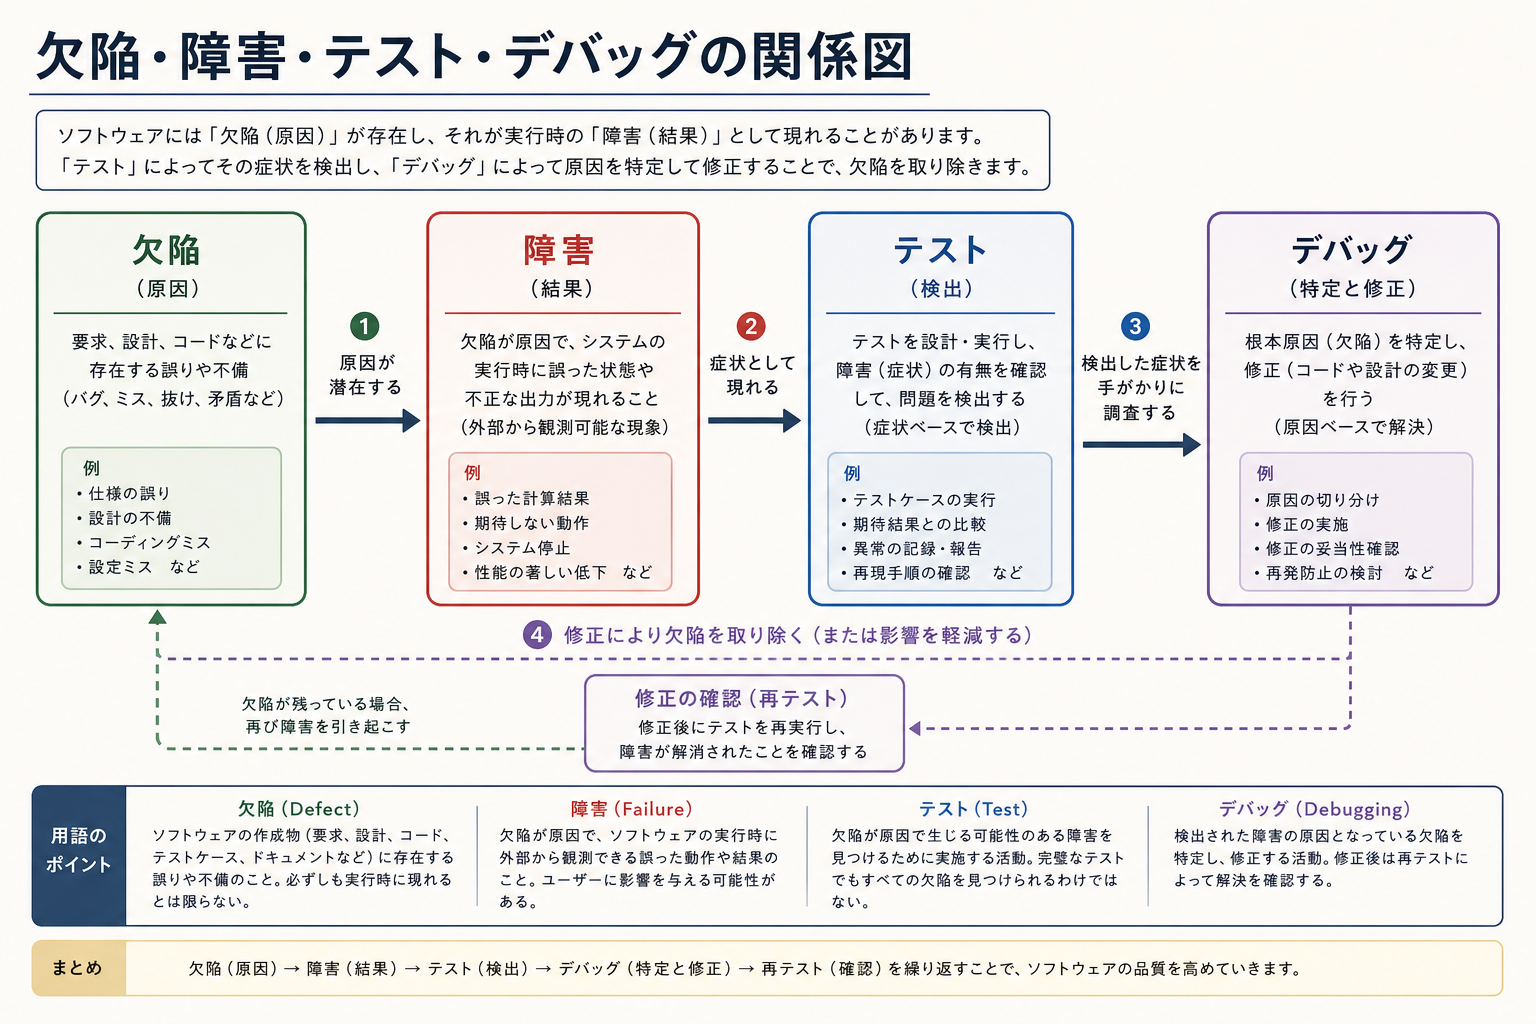
\includegraphics[width=0.96\linewidth]{assets/fig-ch05-03.png}}{\fbox{\parbox[c][48mm][c]{0.9\linewidth}{\centering 画像生成待ち\\欠陥・障害・テスト・デバッグの関係図}}}
\caption{欠陥・障害・テスト・デバッグの関係図}
\label{fig:ch05-03}
\end{figure}
